\section{Results}
\label{sec:results}

\subsection{General Performance}

Overall, our 72 runs showed a wide range of results. We saw everything from near-perfect classification to complete model failure. The best performance came from VGG19 using Adam and Adamax at a learning rate of $10^{-4}$, both reaching an AUC of 0.9995. On the other end of the spectrum, we had 10 "degenerate" runs where the model failed to learn anything useful and just predicted one class for every image.

\subsection{Top Performers}

When we look at the best model for each architecture (Table~\ref{tab:best-arch}), we see that every base model is capable of high performance if given the right optimizer. VGG19 and DenseNet121 both hit very high AUC scores with Adam, while ResNet50 and EfficientNetB3 performed best with RMSProp.

\begin{table}[H]
  \centering
  \caption[Per-Architecture AUC Ranking]{Top configurations for each architecture (ranked by AUC).}
  \label{tab:best-arch}
  \begin{tabular}{llllr}
    \toprule
    \rowcolor{tableheader}
    \textbf{Model} & \textbf{Optimizer} & \textbf{LR} & \textbf{Accuracy} & \textbf{AUC} \\
    \midrule
    VGG19          & Adam    & 1e-4 & 77.33\% & 0.9995 \\
    DenseNet121    & Adam    & 1e-4 & 96.76\% & 0.9991 \\
    ResNet50       & RMSProp & 1e-4 & 95.14\% & 0.9943 \\
    EfficientNetB3 & RMSProp & 1e-4 & 84.62\% & 0.9841 \\
    \bottomrule
  \end{tabular}
\end{table}

\subsection{The Impact of Learning Rate}

One of our biggest findings was just how much the learning rate matters for transfer learning. As we dropped the learning rate from $10^{-4}$ down to $10^{-6}$, performance took a massive hit across the board. 

At $10^{-4}$, most models converged quickly and performed well. However, at $10^{-6}$, many models stopped improving after just 11 epochs (due to our EarlyStopping callback) because the updates were too small to make any real progress. This tells us that for these specific frozen models, $10^{-4}$ is likely the "sweet spot."

\subsection{Optimizer Comparison}

In our tests, RMSProp was the most consistent performer, with the highest average AUC across all models. Adam and Adamax were also very strong, especially at the $10^{-4}$ learning rate. On the other hand, AdaDelta and SGD struggled significantly on this dataset, especially when combined with smaller learning rates. 

\subsection{Visualizing the Results}

We used heatmaps to visualize how the different architectures responded to the optimizer and learning rate settings. Figures~\ref{fig:heatmap-acc} and~\ref{fig:heatmap-auc} show that while some models are more flexible, most configurations cluster around a specific "ideal" zone in the hyperparameter space.

\begin{figure}[htbp]
  \centering
  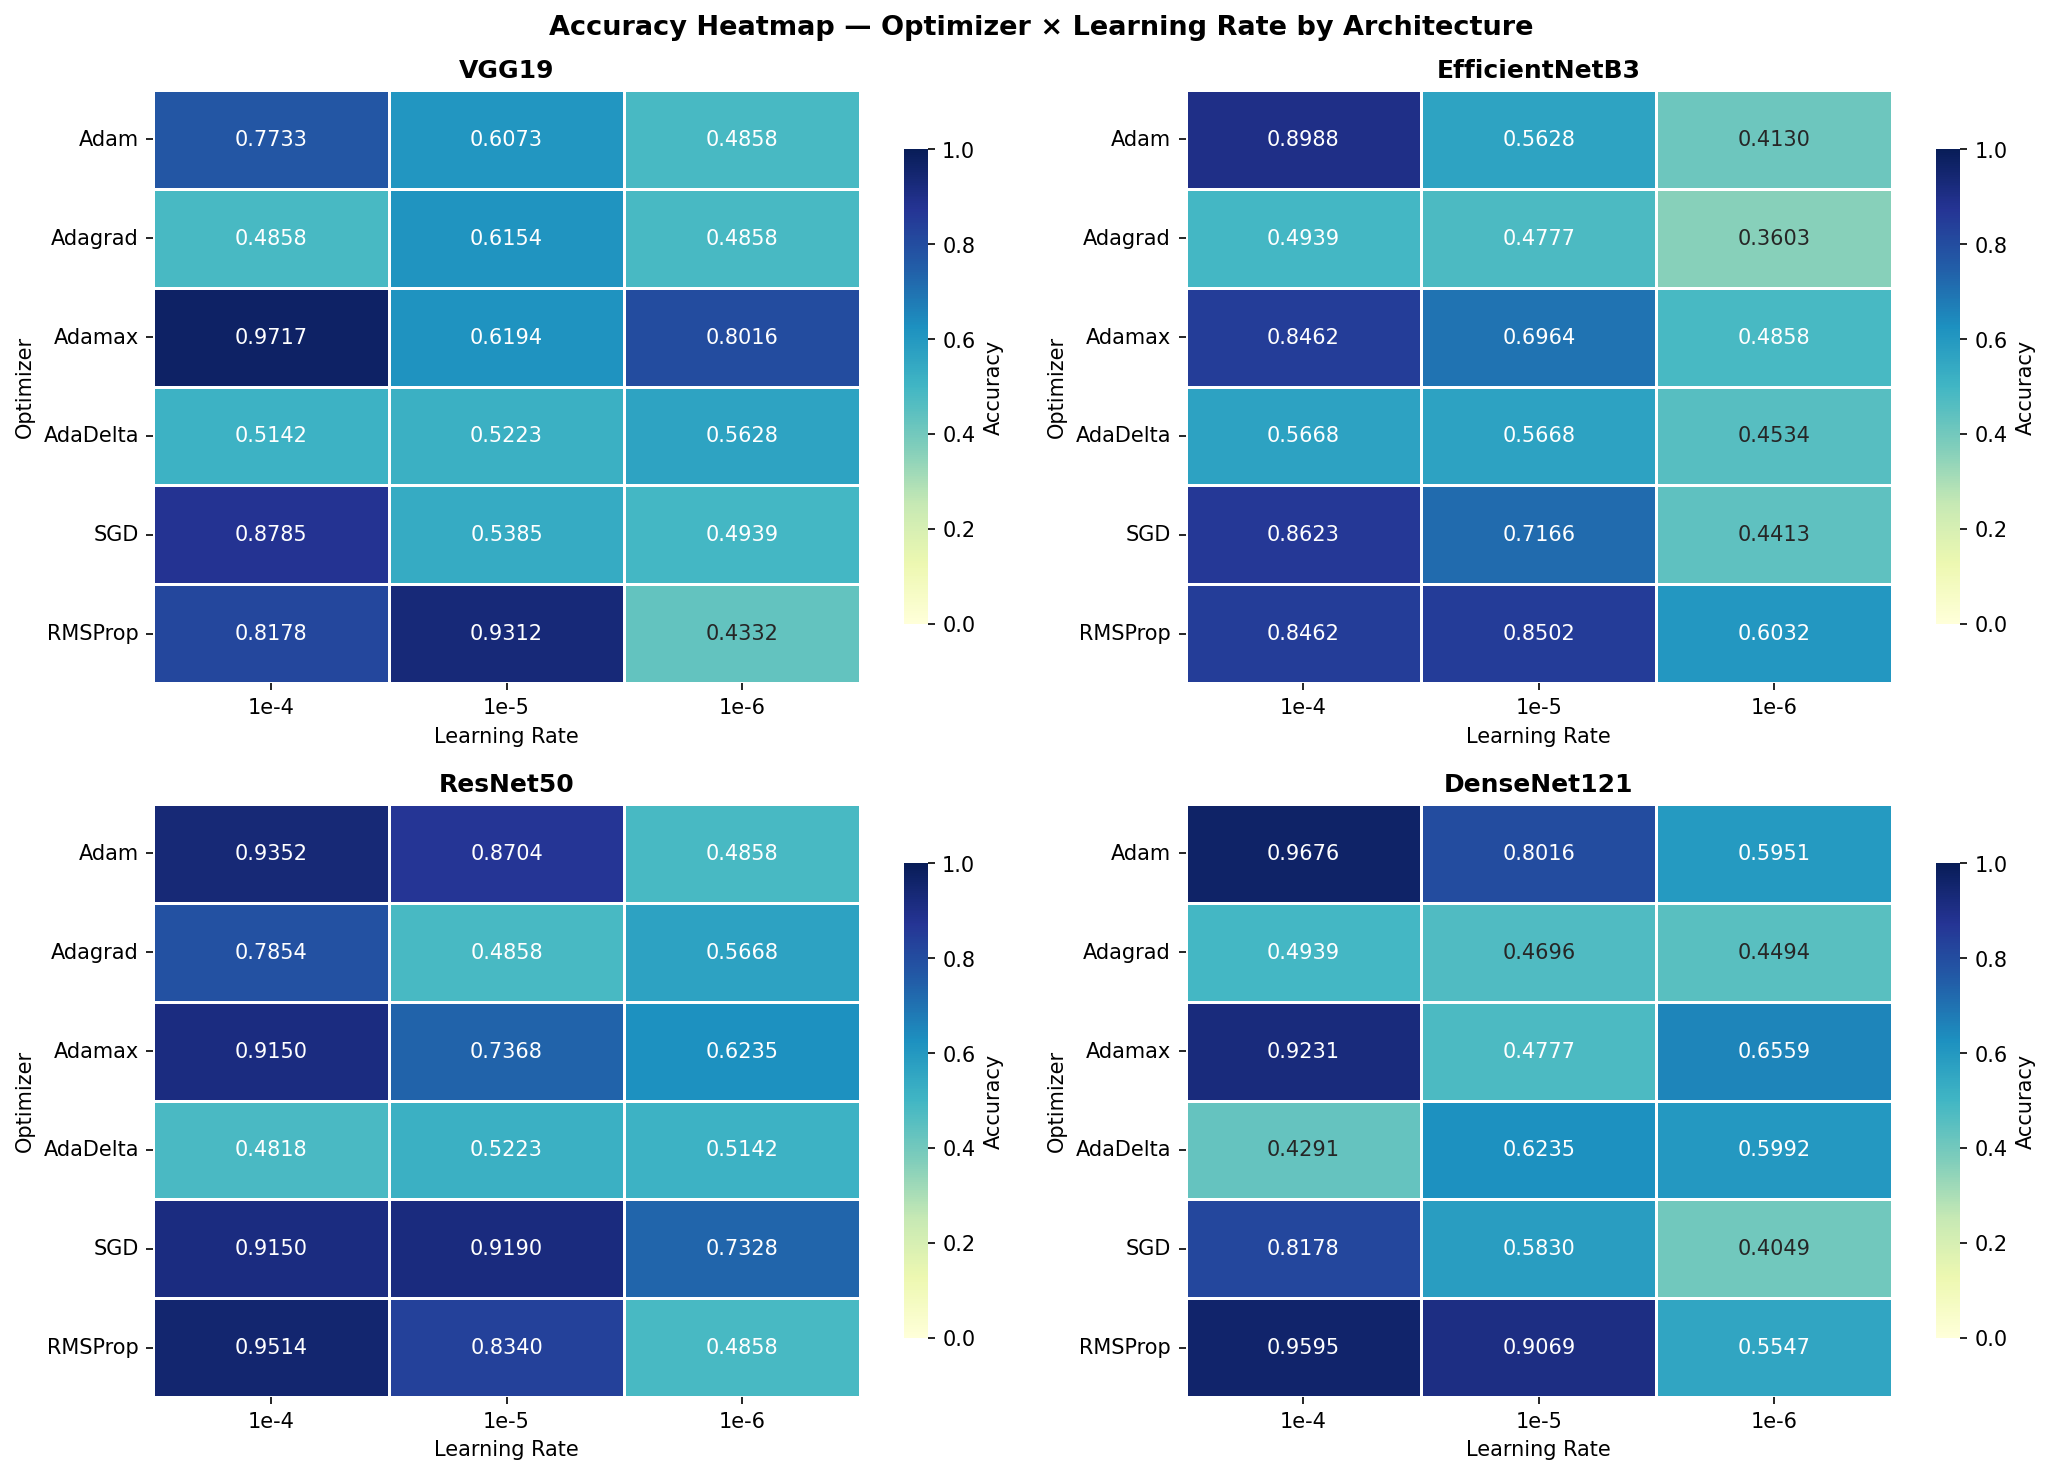
\includegraphics[width=\textwidth]{figures/accuracy_heatmap.png}
  \caption[Full Accuracy Heatmap]{Accuracy across all 72 configurations.}
  \label{fig:heatmap-acc}
\end{figure}

\begin{figure}[htbp]
  \centering
  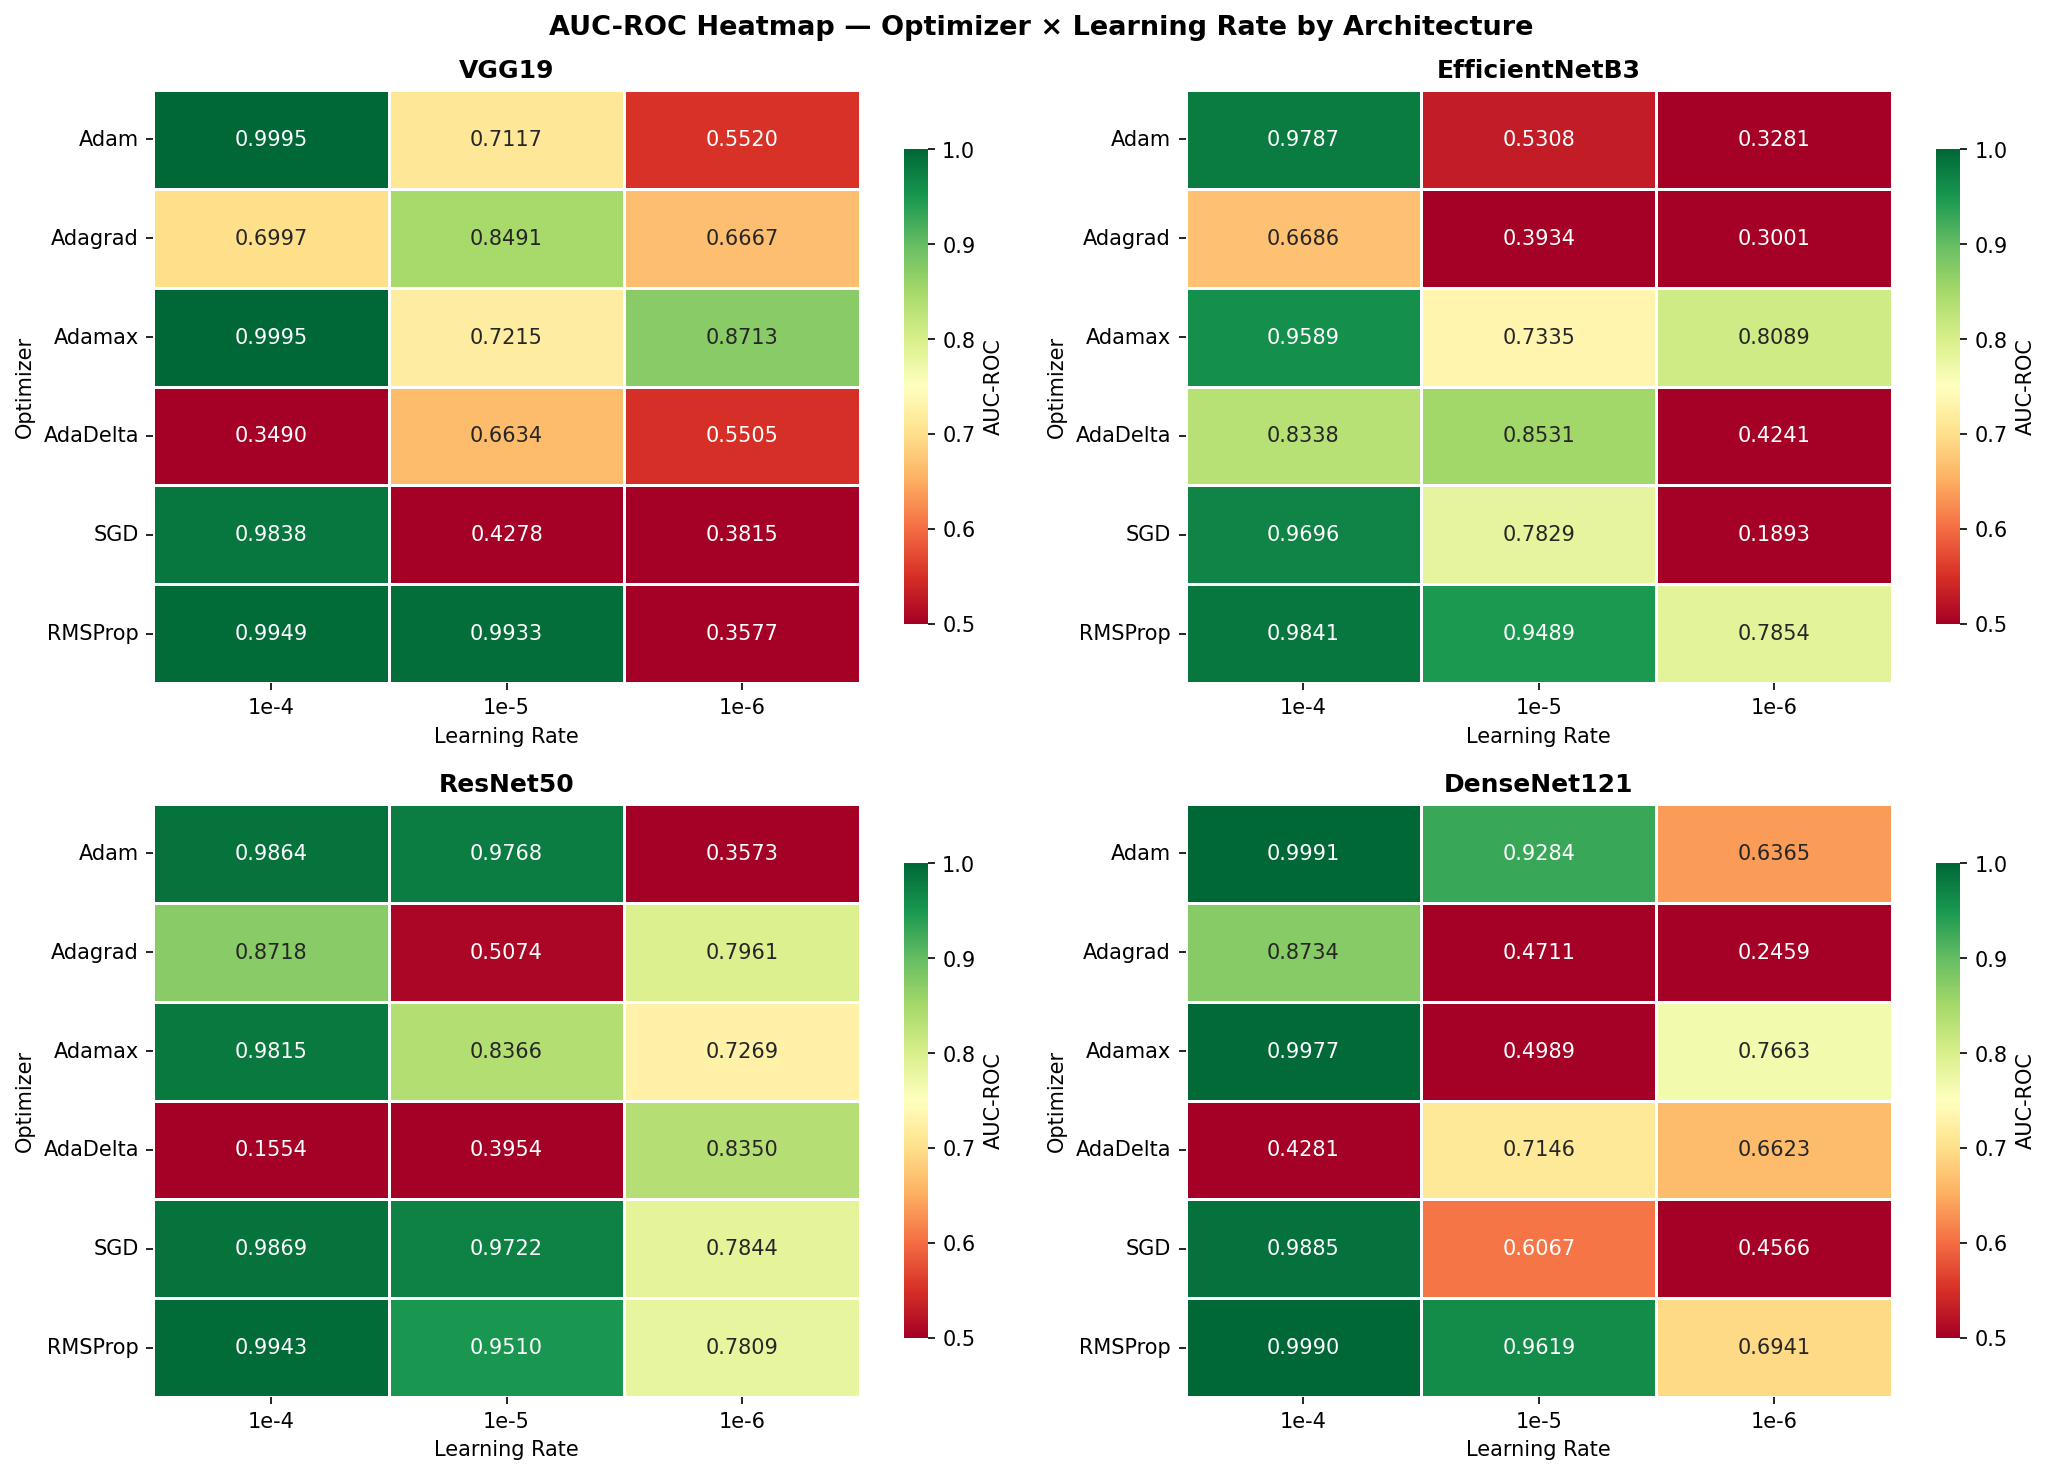
\includegraphics[width=\textwidth]{figures/auc_heatmap.png}
  \caption[Full AUC-ROC Heatmap]{AUC-ROC across all 72 configurations.}
  \label{fig:heatmap-auc}
\end{figure}

\subsection{Failures and Degenerate Runs}

It's also worth noting the runs that failed. We identified 10 cases where the models simply "collapsed" to predicting one class. Interestingly, some of these runs still showed a high AUC (above 0.80) even though they were practically useless because they never correctly identified a single cancer (or non-cancer) case. This highlighted why we need to look at more than just AUC when evaluating these models for medical use.
